\documentclass[10pt]{article}
\usepackage[
    paperwidth=8.0139in,
    paperheight=6.2739in,
    margin=0in
]{geometry}

\usepackage[T1]{fontenc}
\usepackage{newtxtext,newtxmath}
\usepackage{tikz}
\usetikzlibrary{arrows.meta}
\usetikzlibrary{calc}

\pagestyle{empty}
\begin{document}
    \noindent
    \resizebox{8.0139in}{6.2739in}{%
        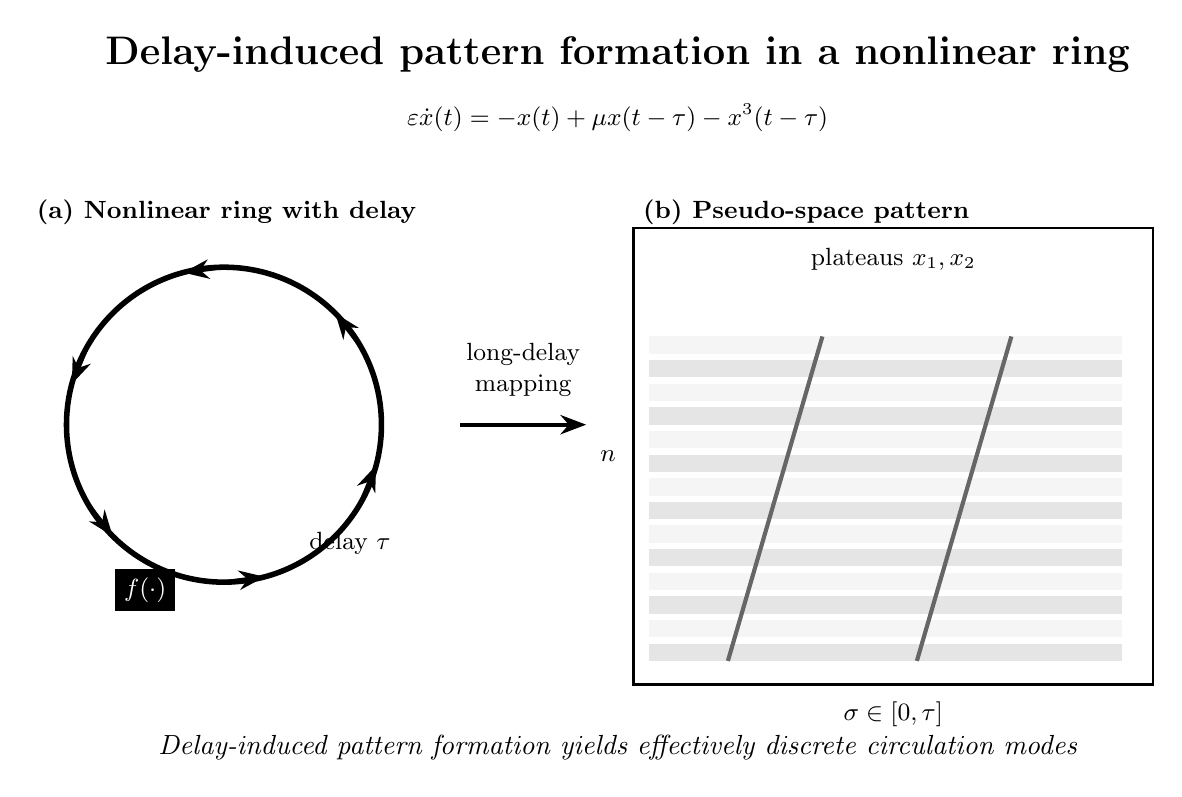
\begin{tikzpicture}[
            font=\small,
            >=Stealth,
            frame/.style={draw=black, line width=0.8pt},
            front/.style={line width=1.5pt, black!60}, % Adjusted for proper visibility
        ]

%------------------------------------------------------------------
% TITLE
%------------------------------------------------------------------
            \node[font=\bfseries\Large] at (8,9.2)
                {Delay-induced pattern formation in a nonlinear ring};

            \node at (8,8.4)
                {$\varepsilon \dot{x}(t) = -x(t) + \mu x(t-\tau) - x^3(t-\tau)$};

%------------------------------------------------------------------
% LEFT PANEL: ring with delay
%------------------------------------------------------------------
            \node[anchor=west] at (0.5,7.2) {\bfseries (a) Nonlinear ring with delay};

            \draw[line width=2pt] (3,4.5) circle (2);

            \foreach \a in {30,90,150,210,270,330} {
                \draw[->,line width=1.4pt] ({3+2*cos(\a)},{4.5+2*sin(\a)})
                -- ({3+2*cos(\a+15)},{4.5+2*sin(\a+15)});
            }

            \node[draw, fill=black, text=white, inner sep=3pt] at (2,2.4) {$f(\cdot)$};
            \node at (4.6,3.0) {delay $\tau$};

%------------------------------------------------------------------
% ARROW
%------------------------------------------------------------------
            \draw[->,line width=1.4pt] (6,4.5) -- (7.6,4.5);
            \node[align=center] at (6.8,5.2) {long-delay\\mapping};

%------------------------------------------------------------------
% RIGHT PANEL: pseudo-space
%------------------------------------------------------------------
            \node[anchor=west] at (8.2,7.2) {\bfseries (b) Pseudo-space pattern};

            \draw[frame] (8.2,1.2) rectangle (14.8,7.0);

            % Axes labels
            \node[anchor=north] at (11.5,1.1) {$\sigma \in [0,\tau]$};
            \node[anchor=east] at (8.1,4.1) {$n$};

            % Alternating plateau bands (Shaded regions)
            \foreach \y/\c in {
                1.5/10,1.8/4,2.1/10,2.4/4,2.7/10,
                3.0/4,3.3/10,3.6/4,3.9/10,
                4.2/4,4.5/10,4.8/4,5.1/10,5.4/4
            }{
                \fill[black!\c] (8.4,\y) rectangle (14.4,\y+0.22);
            }

            % CORRECTED: Drifting fronts (Continuous domain walls)
            % These lines now track the exact drift velocity of the transition fronts
            \draw[front] (9.4, 1.5) -- (10.6, 5.62);
            \draw[front] (11.8, 1.5) -- (13.0, 5.62);

            \node at (11.5,6.6) {plateaus $x_1,x_2$};

%------------------------------------------------------------------
% CAPTION TAGLINE
%------------------------------------------------------------------
            \node[font=\itshape] at (8,0.4)
                {Delay-induced pattern formation yields effectively discrete circulation modes};

        \end{tikzpicture}
    }

\end{document}